\chapter{Vesting System}

\section{Introduction}

In this chapter, we present a model for the vesting schedule domain-specific language (DSL). A vesting schedule is a contractual agreement between an employer and an employee that governs the employee's right to receive equity or other forms of compensation over time. The vesting schedule typically consists of a series of vesting periods during which the employee earns the right to receive a portion of their equity or compensation. The vesting periods are governed by a set of conditions and triggers, which determine when the employee is entitled to receive their equity or compensation. The vesting schedule DSL provides a way to express these conditions and triggers in a formal language, allowing us to reason about and analyze vesting schedules more easily. In this chapter, we will present our model for the vesting schedule DSL and discuss its features, including vesting terms, conditions, and triggers, as well as unary and binary operators for composing and manipulating these constructs. We will also present interesting cases and applications of our model.

\section{Model Overview: Vesting Terms, Conditions, and Triggers}

Our model for the vesting schedule DSL is based on three main constructs: vesting terms, conditions, and triggers.

The preliminaries are giving an ordering to dates, and defining a graph for vesting triggers, so we can make them well-formed (i.e., acyclic, since they are like an abstract syntax tree).

\begin{listing}[!h]
\begin{minted}{alloy}
open util/ordering[Date]
open util/graph[VestingTrigger]

sig Date {}
\end{minted}
\caption{The \texttt{Date} signature}
\label{lst:date-signature-3}
\end{listing}


A vesting term represents a period of time during which an employee earns the right to receive a portion of their equity or compensation.

\begin{listing}[!h]
\begin{minted}{alloy}
abstract sig VestingTerm {
    conditions : disj set VestingCondition,
    shares : one Int
}
\end{minted}
\caption{The \texttt{VestingTerm} signature}
\label{lst:vesting-term-signature-3}
\end{listing}


A vesting condition represents a condition that must be satisfied for the employee to earn the right to receive their equity or compensation.

\begin{listing}[!h]
\begin{minted}{alloy}
abstract sig VestingCondition {
    trigger : disj one VestingTrigger,
    shares : one Int,
    term : one VestingTerm
}
\end{minted}
\caption{The \texttt{VestingCondition} signature}
\label{lst:vesting-condition-signature-3}
\end{listing}


Finally, we defined abstract triggers before giving the concrete cases.

\begin{listing}[!h]
\begin{minted}{alloy}
abstract sig VestingTrigger {}

abstract sig UnaryOperator extends VestingTrigger {
    operand : one VestingTrigger
}

abstract sig BinaryOperator extends VestingTrigger {
    left : disj one VestingTrigger,
    right : disj one VestingTrigger
}
\end{minted}
\caption{The \texttt{VestingTrigger} signature}
\label{lst:vesting-trigger-signature-3}
\end{listing}


% Add a picture from pics/vesting-system.png
\begin{figure}[ht]
\centering
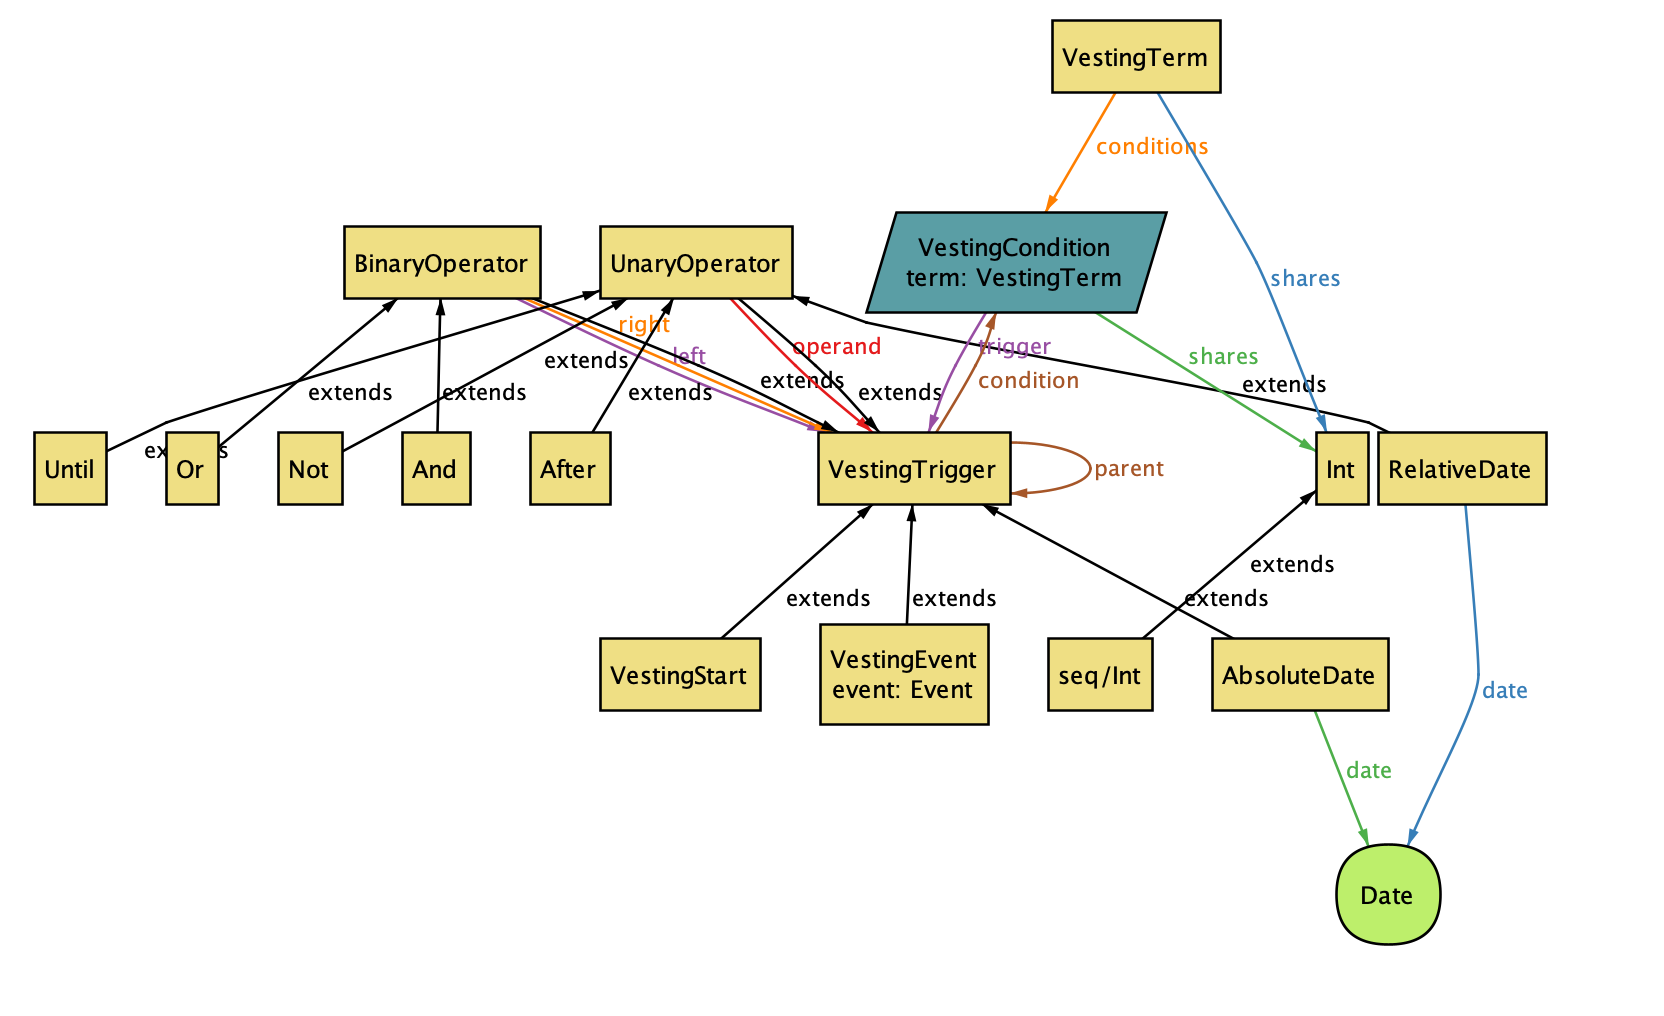
\includegraphics[width=0.8\textwidth]{pics/vesting-system.png}
\caption{Vesting system}
\label{fig:vesting-system}
\end{figure}

\section{Unary and Binary Operators: Until, After, Not, And, and Or}

In addition to the basic vesting triggers described previously, our vesting schedule DSL also includes a number of unary and binary operators that can be used to combine and modify these triggers to create more complex vesting schedules.

\subsection{Unary Operators}

Unary operators are operators that operate on a single trigger. In our DSL, we have defined three unary operators: Until, After, and Not.

\subsubsection{Until}

The Until operator is a unary operator that modifies a trigger to only trigger until a certain date. In Alloy, we define the Until operator as follows:

\begin{listing}[!h]
\begin{minted}{alloy}
sig Until extends UnaryOperator {
    date : one Date
}
\end{minted}
\caption{The \texttt{Until} signature}
\label{lst:until-signature}
\end{listing}



This operator can be used to model vesting conditions that expire on a certain date, or that can only be exercised within a certain time period.

\subsubsection{After}

The After operator is a unary operator that modifies a trigger to only trigger after a certain date. In Alloy, we define the After operator as follows:


\begin{listing}[!h]
\begin{minted}{alloy}
sig After extends UnaryOperator {
    date : one Date
}
\end{minted}
\caption{The \texttt{After} signature}
\label{lst:after-signature}
\end{listing}


This operator can be used to model vesting conditions that cannot be exercised until a certain date.

\subsubsection{Not}

The Not operator is a unary operator that negates a trigger. In Alloy, we define the Not operator as follows:

\begin{listing}[!h]
\begin{minted}{alloy}
sig Not extends UnaryOperator {}
\end{minted}
\caption{The \texttt{Not} signature}
\label{lst:not-signature}
\end{listing}


This operator can be used to model vesting conditions that are contingent on the absence of certain events or conditions.

\subsection{Binary Operators}

Binary operators are operators that operate on two triggers. In our DSL, we have defined two binary operators: And and Or.

\subsubsection{And}

The And operator is a binary operator that combines two triggers into a new trigger that only triggers if both triggers are true. In Alloy, we define the And operator as follows:

\begin{listing}[!h]
\begin{minted}{alloy}
sig And extends BinaryOperator {}
\end{minted}
\caption{The \texttt{And} signature}
\label{lst:and-signature}
\end{listing}


This operator can be used to model vesting conditions that are contingent on multiple events or conditions.

\subsubsection{Or}

The Or operator is a binary operator that combines two triggers into a new trigger that triggers if either trigger is true. In Alloy, we define the Or operator as follows:

\begin{listing}[!h]
\begin{minted}{alloy}
sig Or extends BinaryOperator {}
\end{minted}
\caption{The \texttt{Or} signature}
\label{lst:or-signature}
\end{listing}


This operator can be used to model vesting conditions that are contingent on either of multiple events or conditions.

By combining these unary and binary operators with the basic vesting triggers described earlier, we can create complex vesting schedules that model a wide range of vesting conditions.

